% Created 2018-07-12 Thu 14:29
\documentclass[12pt, letterpaper]{paper}
\usepackage[utf8]{inputenc}
\usepackage[T1]{fontenc}
\usepackage{fixltx2e}
\usepackage{graphicx}
\usepackage{longtable}
\usepackage{float}
\usepackage{wrapfig}
\usepackage{rotating}
\usepackage[normalem]{ulem}
\usepackage{amsmath}
\usepackage{textcomp}
\usepackage{marvosym}
\usepackage{wasysym}
\usepackage{amssymb}
\usepackage{hyperref}
\tolerance=1000
\usepackage{minted}
\usepackage{natbib}
\usepackage[margin=1in]{geometry}
\def\BigO{{\cal O}}
\author{Timothy Schwieg}
\date{\today}
\title{Outline}
\hypersetup{
  pdfkeywords={},
  pdfsubject={},
  pdfcreator={Emacs 25.3.1 (Org mode 8.2.10)}}
\begin{document}

\maketitle

\section{Data}
\label{sec-1}
The are from the steam community market and concern most of the items
that can be bought and sold at market. Almost all items in
counter-strike are trade-able, although some restrictions exist. These
restrictions can take the form of no-trade periods on certain items
after purchase as well as certain items related to esports are
untradable. In short, the market is modeled by a continuous double
auction. Each item sold has a quality attributed to it that is
distributed uniformly on the unit interval; these qualities are broken
down into several classes and each of those are sold separately on the
market.

Even though buy and sell orders are placed, and are used to
facilitate the exchanges between the participants, the seller's price
is always paid. Without considerations of dynamics, this would mean
that the buyer faces a dominant strategy of revealing his valuation
when placing his bid. However the effects of the seller shading is
likely minimal since this is a very large online double auction,
and is converging to the competitive equilibrium very quickly.

The data collected take three forms: first, price and
quantity history data taken from market transactions. Within the last
thirty days hourly data exists on the median price and quantity of items
sold at the market. There is no specific buy and sell order data
for these transactions. This complication makes estimating the model
as a double auction difficult. There is no data on the specific buy
and sell orders made, even the winning ones. All that is recovered is
the price and the quantity. The structure of the auction, where the
seller's price is paid means that we do observe the seller's bids, but
not the buyer's bids. Only the median price is observed, not
the actual price of all transactions occurring within that hour. This
means that there is some error, but since it is pretty negligible it
will just have to be ignored.

The other forms the data take are the outstanding buy and sell orders
in the market. These are buy and sell orders that have gone
unfulfilled so far. They make up about a third of the data for most of
the items on the market. These data are more useful as the
only part of the data that are the actual bids. These data are split into
two parts, the buy orders and the sell orders, each of which has the
price and the cumulative number of buy orders that would be willing to
purchase at this price. The fact that this gives us separate supply
and demand only data points should help during
identification. 

\section{Model}
\label{sec-2}

For any given item, assume that there is a mass of consumers who have
valuations based on some distribution $F_V$. With some exogenous
probability, some consumers are endowed with an item with probability
$p$. Consequently, the same distribution of valuations in those
endowed as well as those who are not endowed, even if there are
different numbers of people who are endowed. 

Because the process of granting items is random, it is in no way
efficient. No process exists that leads to the individuals who
value the good most receive it under the current function. In order to
achieve this efficiency, a market is implemented, taking the form
of a double auction.

It is known that double auctions  converge rapidly to a competitive
enviorment. The data pulled are relatively poor for extracting
valuations from the bids, as for much of the data the bids are not
observed; as a result attempting to identify valuations from the bids
would not work well. Even though the result is certainly possible for
double auctions under conditions such as sealed-bid, and one buyer and
seller, there has been no identification, based on a dominant or
equilibrium argument in the continuous double auction. 

Consequently, I shall abstract from the dynamics and the
mechanism of the double auction, and due to the large amount of
traffic, focus on its convergence into a competitive market. If the
market is efficient, then a matching between buyers and
sellers obtains after the trades where those with the highest
valuations have the items.

\subsection{The Matching Problem}
\label{sec-2-1}
Since it is known that the planner's problem of maximizing total
welfare, and the decentralized market are equivalent for this problem,
one can examine either interchangeably to provide context for the
problem.

The surplus generated by any exchange between a buyer and a seller is
given by the valuation of the buyer minus the valuation of the
seller. A central planner, who wishes to maximize the total surplus
then faces the question of finding a path between the Cartesian
product of buyers valuations and sellers valuations that maximizes:

This process simplifies to a continuous linear program. Even though
this LP has a solution and a duality gap of zero, it is quite unwieldy
to work with. It is easier to consider a discretised alternative:
breaking the distribution of valuations into discrete chunks. Instead
of a distribution of types of buyers and sellers, there are finitely
many, which represent the mass that is contained in their
quantiles. One major advantage of this approach is that it is very
simple to handle the question of there being different numbers of
buyers and sellers. Under the continuous linear program, one
would have to ensure that the manifold was measure-preserving after
controlling for the percent of the population who has the item, in the
case of the discrete version, one only has to increase or decrease the
number of buyers or sellers. 

Under the discrete model, I consider $I$ quantiles of the valuations
for the buyers, and $J$ quantiles of the valuations for the sellers. The
valuations are therefore given by the inverse distribution function
applied to the index of the buyer divided by $I$, or the index of the
seller divided by $J$. The linear program for discrete planners problem
is as follows:

\begin{align*}
\max_{\alpha_{i,j}} & \sum_{i=1}^I \sum_{j=1}^J \left [ F_V^{-1} \left ( \frac{i}{I} \right ) - F_V^{-1} \left ( \frac{j}{J} \right ) \right ] \alpha_{i,j }\\
\text{subject to: } & \forall j, 1 \leq j \le J \quad \sum_{i=1}^I \alpha_{i,j} \leq 1 \\
& \forall i, 1 \leq i \leq I \quad \sum_{j=1}^J \alpha_{i,j} \le 1 \\
\end{align*}

The constraints serve to require that each individual make at most
one exchange. Of interest as well is the dual of the problem, which is
specified below.

\begin{align*}
\min_{x,j} & \sum_{i=1}^I x_i + \sum_{j=1}^J y_j \\
\text{subject to: } & \forall i,j; \quad 1 \leq j \leq J, \quad 1 \le i \leq I\\
& x_i + y_j \geq F_V^{-1} \left ( \frac{i}{I} \right ) - F_V^{-1} \left ( \frac{j}{J} \right ) 
\end{align*}

The solution to this problem form the shadow prices of the exchange,
or the amount of surplus that a buyer or seller takes based on his or
her type. 

\subsubsection{Results}
\label{sec-2-1-1}
One important thing to note about the objective function is that
despite the transformation of the inverse cdf, it remains the buyer's
valuation less the seller's valuation, and this function is both
super-modular and sub-modular. This implies that for this matching
problem, both positive assortative mating and negative assortative
mating are supported. After some inspection, one can see that even though
the process will determine which of the sellers and buyers
match, any permutation of the matches is just as optimal.

That said, the dual of the problem does have a unique solution, as it is
the shadow price for the type of the seller and the buyer. These
values are the producer and consumer surplus for each type. Since it is
a competitive equilibrium, there is one price supported, as the good
is homogeneous, and the matching is occurring between valuations for the
good. The seller's valuation plus his shadow price will be equal to
the competitive price for all sellers who do exchange. 

For equal-sized buyer and seller valuations, this gives the intuitive
result that the lower half of the distribution of sellers will sell to
the upper half of the distribution of buyers, and we will have the
efficient result. As the size of the seller's mass shrinks, with the
rarity of the item increasing, more of the sellers choose to sell, and
the receiving end of the distribution of buyers shrinks, as the price
increases. This is demonstrated below for valuations that are
distributed normally, with mean 35, and standard deviation of 10. The
equilibrium price is calculated by taking the seller's valuation plus
his shadow price. 

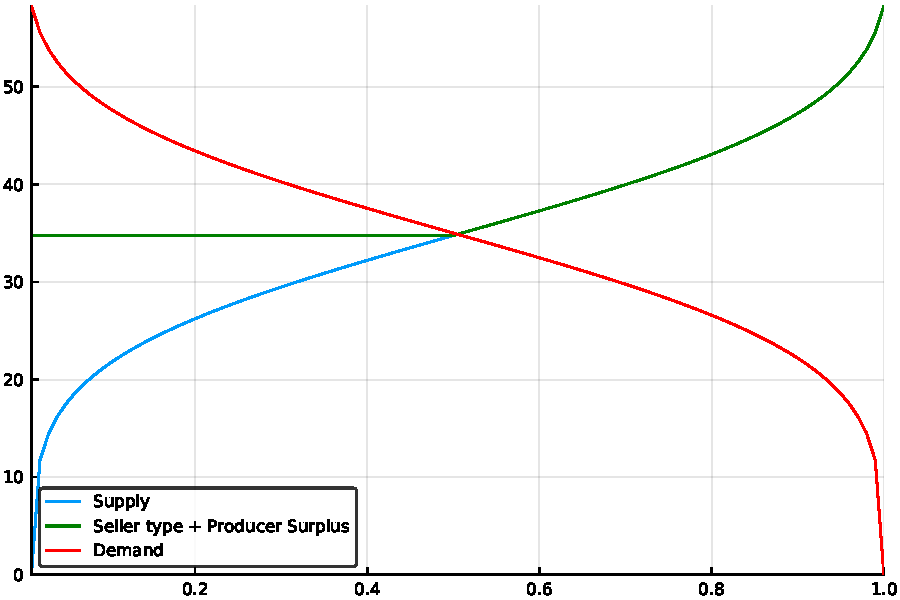
\includegraphics[width=.9\linewidth]{../Scripts/evenStevens.pdf}

If one considers the decentralized market version of the problem, all
buyers are indifferent between the sellers they choose, as they must
give up the producer surplus to the seller, and as a result face a
constant price to buy from any seller type. 

When the proportion of the population are buyers is increased to ten
times the proportion of the population that are sellers, we see the
result change:

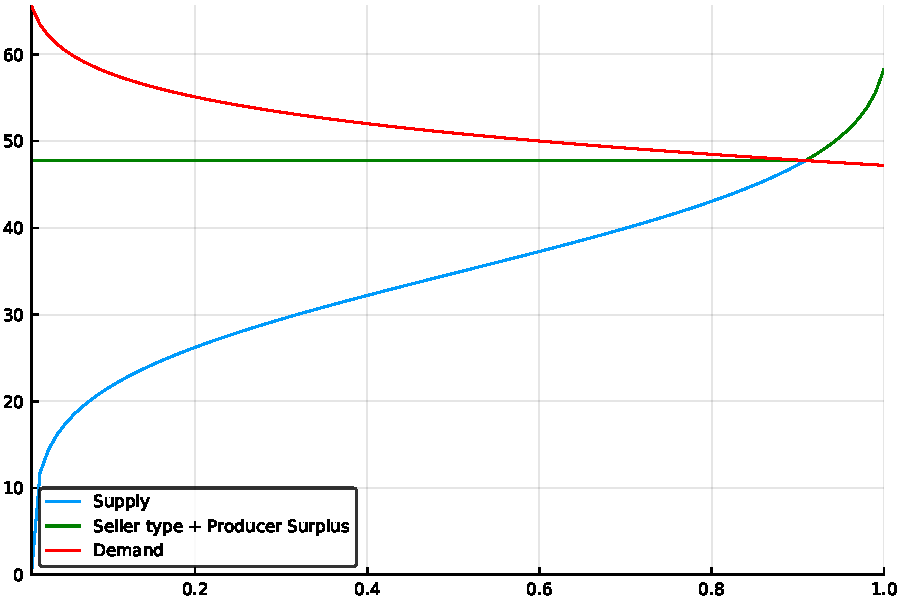
\includegraphics[width=.9\linewidth]{../Scripts/oneTenth.pdf}

The distribution of buyers has become truncated by the difference in
the number of buyers and sellers. To maintain the efficient outcome,
only the top $10$ percent of the buyers are able to purchase, and $90$
percent of the sellers are now selling. The result is a much higher
price.

While we would want to put down this change in the price to constant
demand, but a decrease in supply, the distribution of sellers has
remained constant, and in fact more of them are selling now. Within
the context of this matching model, the change in the relative sizes
of the population of suppliers acts to truncate the buyers rather than
lower the supply. It is important to note that these are not exactly
supply and demand in the normal sense, as instead of quantity, the
$x$-axis is the proportion of the sellers that exchange.

\subsubsection{Equilibrium}
\label{sec-2-1-2}
As a result of the lens in which this market is viewed, a slightly
different sort of equilibrium obtains. Although all the desirable
properties of an equilibrium hold, notably efficiency, and being in
the core, we are only examining exchanges in one good, so it remains a
partial equilibrium.

Assume that the valuations of the players are distributed
normally, as in the examples above. Then the supply function can be
written as $q = \Phi \left ( \frac{ p - \mu }{\sigma} \right )$ and the demand
function can be written as: $q \left ( \frac{\xi}{1-\xi} \right ) = 1 - \Phi \left ( \frac{
p - \mu }{ \sigma } \right )$, $\xi$ is the percent of people endowed with
the item. In equilibrium, the quantity of buyers and sellers are
equal:

\begin{align*}
\Phi \left ( \frac{ p^* - \mu }{\sigma} \right ) &= \frac{1-\xi}{\xi} \left [ 1 - \Phi \left
( \frac{ p^* - \mu }{\sigma} \right ) \right ]\\
p^* &= \mu + \sigma \Phi^{-1} ( 1- \xi )\\
\end{align*}

Which tells us the price that the market supports is the average
valuation plus a component that depends on the rarity of the
item. Essentially this claims that the price is controlled by some
universal notion of value, such as the design of the skin, as well as
a rarity element that drives price up or down depending on how easy it
is to obtain.

\subsection{Identification}
\label{sec-2-2}
For some fixed $\xi$, this model gives a deterministic price for some
distribution of valuations. If one were to claim that the randomness in
this model arises from some unobserved error, then it remains
unidentified: $p^* = \mu + \sigma \Phi^{-1} ( 1 - \xi) +
U$. Three primitives exist, but any estimates of the price would
only have a single dimension. No published numbers of $\xi$ exists, and
the mechanism for determining it is complicated at best.

\subsubsection{Estimating $\xi$}
\label{sec-2-2-1}

If one were able to estimate $\xi$, then the problem becomes one of
regression, and the covariates suffer from measurement error. This
would lead to biased and inconsistent estimates of the
coefficients. Clever rearrangement of the model might allow for
estimation, it is quite difficult to estimate $\xi$ outside of the
model. Crude estimates of $\xi$ may be able to be obtained using the
number of creates sold and the probabilities of each item being
unboxed by the item. However there are several complications that make
this almost impossible to handle.

\begin{itemize}
\item No data concerning the actual inventories of active
players exists. Players are able to set their inventories as private,
preventing anyone from seeing their contents.
\item Items can be combined into other items of higher quality, and there
is no data on the percentage of times this has been done.
\item The actual drop rate of the items is unknown, and the amount of
possible drops is limited to a only two per week per player. There
are no reliable estimates of the drop rate, nor what factors affect
it.
\end{itemize}

Since rare items are obtained almost exclusively through opening loot
boxes, one could obtain an estimate of the percentage of people
endowed with the item by taking the number of the lotteries sold and
multiplying it by the probability of obtaining that particular item in
the lottery. However the error cannot be quantified, and any
regression coefficients remain biased and inconsistent.

\subsubsection{Another Estimation Strategy}
\label{sec-2-2-2}

If all estimates of $\xi$ are unsatisfactory, as I believe, then one
method of estimating $\mu$ and $\sigma$ is to allow the deviations in the price
not be caused by random additive shocks, but instead by randomness
contained within $\xi$. By assuming a distribution on $\xi$, one may admit for
the randomness in the price, even when all other covariates contained
in the mean do not change. Effectively, we buy identification by
taking a very strong stance on how the endowments are distributed
among the population, and that all the noise in the price is caused by
these deviations in the distributions.

Computationally, this result is not very clean, unless it happens
that the distribution is uniform on the entire unit interval, the
distribution of $p$ will not take a very "nice" form. Effectively, this
identification assumption has quite a lot of power in determining the
form of the valuations, and calls for a very strong assumption on the
nature of $\xi$. However, as stated above, there is very little
information known about $\xi$, as it is unobserved, and taking a strong
stance about the nature of it is at best guess-work. 

\subsubsection{Using the Quantity sold to approximate}
\label{sec-2-2-3}

All of the calculations so far have only used the price data, but one
may be able to use the quantity sold for a useful calculation. Since
the amount that is sold is determined solely by the percentage of the
population that receives the item, and the distribution is important
only for calculating the price that the item costs, one may use the
quantity of an item sold divided by the number of active players to
determine the percentage of the population that has
exchanged. Although this cannot account for exchanges that did not
take place on the market, it is still the best estimate that can
likely be gathered from the data.

For each item sold, there are different qualities
sold at market, and the probability of obtaining each quality is
known, one may form the estimate for each of the different
qualities. This allows us several values of $\xi$ observed, for which we
will have to assume that the mean is constant. However, this forces a
zero restriction of quality on the mean of the valuations, which is a
rather unreasonable assumption. By approaching the model this way, it
claims that the differences in prices between the different qualities
of items is driven solely by the probability of them being
dropped. This is unreasonable. Any attempt to put indicators for the
quality inside the mean will cause there to be colinearity in the
covariates, and linear regression will not produce a result. 
If however, we are willing to accept this mispecification error as
small enough to not cause problems, or if we only examine the highest
qualities among which there is almost no discernible difference, we
can estimate this model using linear regression. 

Since only the drop rate will be measured will be measured with error,
we need only rearrange the regression so that the drop rate is the
dependent variable, for which measurement error does not induce bias
and inconsistency. The estimable model would then be:

\begin{align*}
\Phi^{-1} ( 1- \xi ) = \frac{p^*}{\sigma} - \frac{\mu}{\sigma} \\
\Phi^{-1} ( 1- \xi ) = \beta_0 + \beta_1 p^* \\
\end{align*}

This method can be estimated using linear regression, and the values
of $\beta$ can be adjusted to determine the true values of the $\mu$ and $\sigma$ for
the distribution. All these results are driven by forcing the
quality to have no effect on the mean, and the magnitude of this error
cannot be observed. What we would like to seek is another way to
observe changes in $\xi$ that does not require such a strong assumption.

\subsection{Dynamic Approach}
\label{sec-2-3}
One possible way to handle the identification is to use the only
covariate that has a zero restriction on the mean: time. Consider a
series of time intervals, in which there is a matching device. In each
interval, a percentage of the population is awarded the item, and the
matching device functions as above. We may use the same strategy as
above, estimating $\xi$ using the quantity sold over the total number of
players in the time interval, and this in fact may be more precise
than the estimate used above. However this number can change over
intervals, giving us the changes in $\xi$ needed to identify the mean and
the standard deviation in our model.

First consider the model with no entrants. After the initial
exchange, those that do not have the item are random attributed the
item again, but their distribution is no longer the initial
distribution, it has been conditioned on losing the top portion of its
mass. Therefore the distribution of those that are possible sellers is
a mixture of this truncated distribution, and the top portion that
left the potential buyers. In this model, the top portion of
those that have the item will never sell it, as the valuations of
those that do not are all strictly below them: consider the
seller distribution to be a percentage of the buyers. The process then
repeats, albeit with a slightly truncated portion of the valuation
function. 

This model also more captures more elements of the market than the
original, as it can explain the behavior observed of a high initial
price, and it slowly dropping to some equilibrium level. With an
explanation of the dynamics of the process in place, we can look at
the entire lifetime of the item, and we only have to control for the
truncation of the valuations for the demand. 

As long as there is no entrance of individuals into the model, the
price will necessarily decrease. For the same valuation function as
previous examples: Normally distributed with $\mu$ = 35, $\sigma$ = 10, with a
drop rate of 0.01 per interval and $N = 1000$, a simulation of the price
over these intervals is plotted below.

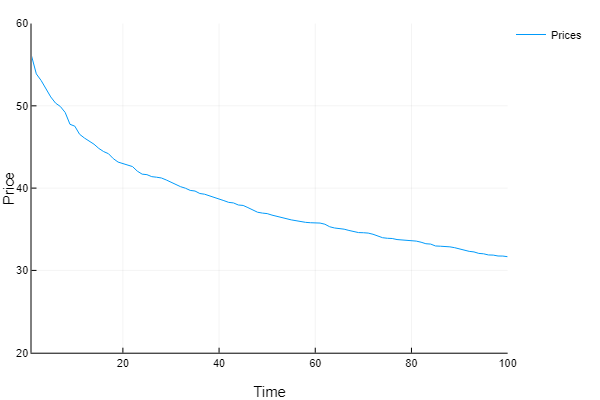
\includegraphics[width=.9\linewidth]{../Scripts/PriceOverTime.png}

One useful result of doing this is that we may be able to get a more
precise estimate of the drop rate, by looking at the number sold in
the first interval that the item was on the market, as it is far less
influenced by exchange and other unobserved factors. This number
divided by the total number of active players will likely give a much
better estimate of the proportion of players who receive the item per
interval.

\subsubsection{Specification}
\label{sec-2-3-1}

Let us be specific with the notation used in this model. For each time
period $t$, the drop rate to individuals estimated is given by: $\xi$$_{\text{t}}$. The
price observed in that period is $p_t$. In the first time period,
everything proceeds according to the previous model. However in the
second time period, allow the top $\xi$$_{\text{0}}$ percent to exit the
model. There are $N(1-\xi_0)$ people remaining, of which $\xi$$_{\text{1}}$ have received
the item, so the mass of suppliers is: $\xi_1 (1-\xi_0)N$. The mass of the
buyers is: $(1-\xi_1)(1-\xi_0)N$. 

\begin{align*}
\Pr \left [ Z < z | Z < F_V^{-1}( 1 - \xi_0 )^{} \right ] &=
\frac { F_V ( z ) }{  F_V ( F_V^{-1} ( 1 - \xi_0 ) ) } = \frac{ F_V (z)
}{1 - \xi_0}\\
q_s &= N ( 1-\xi_0 )\xi_1 \left [ \frac{\Phi \left ( \frac{ p - \mu }{\sigma} \right )}{ 1 - \xi_0 } \right ]\\
q_d &= N ( 1-\xi_0 )(1-\xi_1) \left [ 1 - \frac{ \Phi \left ( \frac{
p - \mu }{ \sigma } \right ) }{ 1 - \xi_0 } \right ]
\end{align*}

We can continue the process, noting that with each truncation, there
is a multiplication of $(1-\xi_t)$ in the denominator of the supply
function.

\begin{align*}
q_s &= N \prod_{t=0}^{T-1} (1-\xi_t ) \xi_T \frac{\Phi \left ( \frac{ p - \mu }{\sigma} \right )}{ \prod_{t=0}^{T-1} ( 1 - \xi_t ) }\\
q_d &= N \prod_{t=0}^{T} ( 1- \xi_t ) \left [ 1 - \frac{ \Phi \left ( \frac{
p - \mu }{ \sigma } \right ) }{ \prod_{t=0}^{T-1} (1 - \xi_t ) } \right ]\\
p^* &= \mu + \sigma \Phi^{-1} \left [ \prod_{t=0}^T ( 1 - \xi_t ) \right ]\\
\prod_{t=0}^T ( 1- \xi_t) = \Phi( \frac{ p^* - \mu }{ \sigma} \\
\end{align*}

Since $\xi$$_{\text{t}}$ is estimated with error, we must still ensure that it appears
in the dependent variable instead of as a covariate, so the model that
we must estimate is as follows:

\begin{align*}
\Phi^{-1 }\left [ \prod_{t=0}^T ( 1 - \xi_t ) \right ] = \beta_0 + \beta_k^T \bold{1}_{\{Quality\}} + \beta_p p^* +
U
\end{align*}

From this, we may obtain our estimates of $\mu$ and $\sigma$, controlling for the
changes in the average valuation caused by the different
qualities. Any other covariates can be added to the model as well, and
controlling whether or not they affect the mean or the standard
deviation by multiplying the indicator by $p^*$. 

\subsubsection{Maximum Likelihood}
\label{sec-2-3-2}

If one believes that assuming the values of $\xi$$_{\text{t}}$ is too strong, another
method is to estimate the different values that it can take by looking
at the distribution of the price, rather than attempting to apply
regression. Consider the distribution function for the price:

\begin{align*}
F_{p^*} = P( p^* < p ) = P( q_s (p) > q_d (p) ) = P( q_d (p) - q_s (p) < 0 )
\end{align*}

Thus knowing the interaction between the distribution of supply and
demand gives us the distribution of price. The distribution of supply
and demand is binomial, as there are N people who can be owners or
purchasers, but the quantity of each are known at each time
period. The distribution of the valuations for each buyer and seller
are given above. Therefore the distribution for the quantity demanded
and supplied is binomial.

In the first time period, there are $N(1-\xi_0)$ buyers, and $N\xi_0$
sellers, and buyers will purchase if their valuations: $\Phi \left (
\frac{ p - \mu }{\sigma} \right )$ are greater than the price, while sellers
will sell if their valuations are less.

\begin{align*}
q_d^0 \sim binom( N (1-\xi_0), 1 - \Phi \left ( \frac{ p -
\mu }{\sigma} \right ))\\
q_s^0 \sim binom( N \xi_0, \Phi \left ( \frac{ p -
\mu }{\sigma} \right )\\
\end{align*}

We may repeat the pattern, using the supply and demand functions above
to determine the distribution of supply and demand in all time
periods.

\begin{align*}
q_d^T \sim binom \left ( N \prod_{t=0}^T ( 1- \xi_t ), 1 - \frac{ \Phi \left ( \frac{ p -
\mu }{\sigma} \right ) }{ \prod_{t=0}^{T-1} ( 1- \xi_t ) } \right )\\
q_s^T \sim binom \left ( N \xi_T \prod_{t=0}^{T-1} (1-\xi_t ), \frac{ \Phi \left ( \frac{ p -
\mu }{\sigma} \right ) }{ \prod_{t=0}^{T-1} ( 1- \xi_t ) } \right )\\
\end{align*}

If we set the expected value of each of these distributions equal to
each other, we arrive at the same pricing condition as
before. However, we are interested in the behavior of: $q_d -
q_s$. Unfortunately, the distribution for the difference between two
binomial distributions is not nicely defined. Instead, since N is very
large, we will use the Normal approximation to the binomial. 

\begin{align*}
q_d^T - q_s^T \sim \mathcal{N} \left \{  N \left [ \prod_{t=0}^T (1 - \xi_t) - \Phi \left ( \frac{ p -
\mu }{\sigma} \right ) \right ], N \big \Phi \left ( \frac{ p -
\mu }{\sigma} \right ) \left [ 1 - \frac{ \Phi \left ( \frac{ p -
\mu }{\sigma} \right ) }{ \prod_{t=0}^{T-1} ( 1- \xi_t ) } \right ] \right \}
\end{align*}

Under
equilibrium, the market price is the closing price, equating supply
and demand. Thus for all the prices seen, we can treat this
distribution as equaling zero, and attempt to maximize the likelihood
of this occurring.

\begin{eqnarray*}
\max & \quad \mathcal{L}( \mu, \sigma, \bold{\xi} )  \\
\text{ subject to: } &\sigma > 0\\
&\xi_i \in [0,1] \quad \forall i\\
&\Phi \left ( \frac{ p_t - \mu }{\sigma} \right ) \geq \prod_{t=0}^T ( 1- \xi_t )\\
\end{eqnarray*}

As it is currently stated, the above problem is not a convex
optimization problem, because of the shape of $\Phi$. As a result it will
be difficult to compute solutions to this problem.

The final feasibility constraint drives that all the prices be
feasible is caused by the partial identification of $\xi$. If we believe
however that there is competitive equilibrium obtained, then the price
in each time period should exactly identify the percent of people that
are buying the item. As a result, all values of $\xi$ are determined
exclusively by the price observed in each period.

\begin{align*}
&\Phi \left ( \frac{ p_t - \mu }{\sigma} \right ) = \prod_{t=0}^T ( 1- \xi_t ) \quad \forall \quad T\\
q_d^T - q_s^T \sim &\mathcal{N} \left \{  0, N \big \Phi \left ( \frac{ p_T -
\mu }{\sigma} \right ) \left [ 1 - \frac{ \Phi \left ( \frac{ p_T -
\mu }{\sigma} \right ) }{ \Phi \left ( \frac{ p_{T-1} - \mu }{\sigma} \right ) } \right ] \right \}
\end{align*}

However, this result creates a serious problem with estimation. As
this model is incapable of realizing the price process increasing, if
we find that $p_t > p_{t-1}$, we will have a negative variance, an
impossibility. One possibility is to add a shock to the system that is
distributed normally as well, large enough that the variance will
always be possible. However in some markets, increasing prices trends
are visible, so the model must be expanding to include this.

\subsubsection{Market Entry}
\label{sec-2-3-3}

Consider the case in which the number of entrants in the market is not
held constant, but new entrants to the market have the same
distribution function as older ones. As a result, the distribution of
the buyers in the following period is now a mixture
distribution. Since we could now find a buyer of the highest
valuation, it is possible that sellers who had previously bought might
be willing to sell again. As a result, the entire seller's
distribution must be considered as well, as a mixture of the highest
portions of demand, and the currently endowed in that instance. 

Consider the model where, after the first exchange of items, $\lambda$$_{\text{0}}$
percent of N people enter the market, drawing their valuations from the original
distribution. Then the endowment process is repeated, and exchange
occurs. After this process, $\lambda$$_{\text{1}}$ percent of the people before the
endowment process enter. That is, $\lambda$$_{\text{t}}$ is the proportion of the
unendowed that enter the market. However, they enter the market after
the exchange has occurred. This ensures that there is no entrance in
the first time period. 

The distribution of buyers and sellers remains binomial. However,
since all sellers are possible sellers now, the mass for the seller's
distribution is noticeably more complex. The mass of the sellers is
now the sum of the mass of the buyers times the percent of people
endowed in each time interval. That is, in time period one, the
sellers received $N \xi_0$ mass, and the mass of the buyers was:
$N(1-\xi_0)$. However, then $\lambda_0$ people arrived, and for time period one
the buyers had mass: $N( 1 -\xi_0 + \lambda_0)(1-\xi_1)$, and the sellers had mass:
$N \xi_0 + N(1-\xi_0 + \lambda_0)\xi_1$. 

The mass of the buyers and the sellers continues on this trend and is
given by:

\begin{align*}
M_B(T) &= N (1-\xi_2 ) \prod_{t=0}^{T-1} ( 1 - \xi_t + \lambda_t ) \\
M_S(T) &= N \sum_{i = 0}^T \xi_i \prod_{t=0}^{i-1} ( 1- \xi_t + \lambda_t )\\
\end{align*}

In each time period, the valuation function evaluated at the price
sold gives the cutoff for the valuations above which the buyer's
purchased, and sellers sold. Taking this into account, the mass of the
buyer and seller can be determined as functions of the valuations and
prices rather than the percent of people who sold:

\begin{align*}
M_B(T) &= N B_T ( p_T )\\
%M_S(T) &= N \left [ B_{k-1}( p_{k-1} ) + \lambda_{k-1} \left [ B_{k-2}(p_{k-2}) + \lambda_{k-2} [...]] - B_k( p_k ) \right ]\\
M_S(T) &= N \left ( 1 - B_T(p_T) + \sum_{t=1}^{T-1}  R_{t}(\lambda,p) \right )\\
R_i(\lambda,p) &= \lambda_i \left [ B_{i-1}(p_{i-1} ) + R_{i-1}(\lambda, p) \right ]\\
R_0 (\lambda,p) &= \lambda_0 \\
\end{align*}

The distribution of valuations has changed for both the buyer and the
seller. When $\lambda$$_{\text{t}}$ people enter the market, the mass of the remaining
people is mixed with the mass of the new entrants. Consider time
period 1, when the first entrants have entered the market. Using the
fact that $B_0 (p_0) = (1-\xi_0)$.

\begin{align*}

P(V_B < p ) &= \left ( \frac{ B_0 ( p_0 ) }{ B_0 (p_0 ) + \lambda_0 } \right )
 \min \left \{ 1, \frac{ B_0 (p) }{ B_0 (p_0 ) } \right \}
 + \left ( \frac{\lambda_0 }{ B_0 (p_0 ) + \lambda_0 } \right ) B_0 (p) \\

P( V_S < p ) &= \left ( \frac{ 1 - B_0 (p_0 )}{ 1 - B_1(p_1 ) + \lambda_0} \right )
 \max \left \{ 0, \frac{ B_0(p) - B_0(p_0 ) }{1 - B_0 ( p_0 ) } \right \}
 + \left ( \frac{ B_0 (p_0 ) - B_1 (p_1) + \lambda_0 }{ 1 - B_1 (p_1) + \lambda_0 } \right ) P( V_B < p )
\end{align*}

In any time period, we can use the fact that $B_T(p_T) = (1-\xi_T ) \prod_{t=0}^{T-1} (1-\xi_T +
\lambda_t )$. This can be used to obtain the distribution function for the
buyer and the seller in all time periods:

\begin{align*}
B_T (p) &= \frac{ B_{T-1 }(p_{T-1}) }{ B_{T-1 }(p_{T-1}) + \lambda_1 } \min \left \{ 1, \frac{ B_{T-1} ( p ) }{B_{T-1 }(p_{T-1 })} \right \}
 + \frac{ \lambda_1 }{ B_{T-1 }(p_{T-1}) + \lambda_1 } B_0 (p) \\
S_T (p) &= \frac{ M_S(T-1) }{ M_S(T) } \max \left \{ 0, \frac{ B_{T-1}(p) - B_{T-1}( p_{T-1} ) }{ 1 - B_{T-1} ( p_{T-1} ) } \right \} + \frac{ M_S(T) - M_S(T-1)_{} }{M_S(T)} B_T (p)\\
\end{align*} 

$B_t(p)$ and $S_t(p)$ are strictly increasing functions of p, so the
intersection between $q_d, q_s$ is uniquely defined. In the case when
$\lambda_t = 0$ this is the dynamic model that we have studied so far.

It is known that the valuations are distributed binomial. Their
difference is approximately distributed normally: 

\begin{align*}
q_d &\sim binom( M_B(T), 1 - B_T(p) )\\
q_S &\sim binom( M_S(T), S_T(p) )\\
q_d - q_s &\sim \mathcal{N}( M_B(T) ( 1 - B_T(p) ) - M_S(T) S_T, M_B(T) ( B_T(p) ( 1 - B_T(p) ) ) +
M_S(T) ( S_T (p ) ( 1 - S_T (p) ) ) )\\
\end{align*}

The estimation problem now has become one of maximizing the likelihood
of the difference between the supply and demand function being equal
to zero. 
% Emacs 25.3.1 (Org mode 8.2.10)
\end{document}